\section{Kings: the Tr\'ebuchet and When It Is Exact}\label{sec:kings}

So far a player with no pawn move simply lost. In chess that player would be stalemated, which is a draw.
Following Elkies~\cite{Elkies1996}, we therefore add the kings in a \emph{tr\'ebuchet}, a king group in mutual
zugzwang that the convention reads as the zero game. In this section we put the kings back on the board and
ask when that reading gives the true chess result. For this we use an exact king-and-pawn solver that plays
real chess: kings, pawns, en passant, all four promotions, stalemate, and no fifty-move rule. An independent
reference solver, written from the rules alone, agrees with it on all $1{,}418{,}480$ positions of its test runs
\lab{C2}, and on the ordinary board we also compare it with the Lichess tablebase~\cite{LichessTB}.

\subsection{Two Tr\'ebuchets}

In Fig.~\ref{fig:trebuchet_2025} the pawns on a4 and a5 block each other, so only the kings can move. The white
king on h5 guards a4 across the seam, and the black king on b4 guards a5. If white (Left) moves first, every king
move gives up a4: the only free square next to a4 that the king can reach, h4, is attacked by the a5 pawn
across the seam. In the same way black (Right), moving first, loses a5, since b5 is attacked by the a4 pawn.
Whichever player goes first will lose a pawn, allowing the other side's pawn to advance and promote. Thus this
position is a zero game. On an ordinary board the king on h5 would not touch a4, so the zugzwang exists only
because of the seam. With the kings played out it is a real mutual zugzwang: with white to move black wins, and
with black to move white wins \lab{C2}.

Fig.~\ref{fig:trebuchet} shows the same idea on files f to h of the ordinary board: the white king's only free
square next to g4, f4, is attacked by the g5 pawn, and the black king's only one next to g5, h5, by the g4 pawn.
The Lichess tablebase confirms that it is a real mutual zugzwang \lab{C2}. This is the king group we place
beside every ordinary-board pawn position in this paper.

\begin{figure}[!t]
\centering
\begin{subfigure}{0.48\columnwidth}
\centering
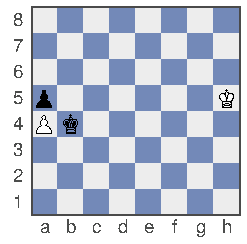
\includegraphics[width=\linewidth]{figures/trebuchet_2025.pdf}
\caption{Kh5, Pa4 / Kb4, Pa5 (cylinder: files a and h adjacent).}
\label{fig:trebuchet_2025}
\end{subfigure}\hfill
\begin{subfigure}{0.48\columnwidth}
\centering
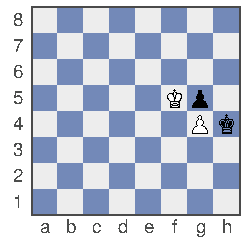
\includegraphics[width=\linewidth]{figures/trebuchet.pdf}
\caption{Kf5, Pg4 / Kh4, Pg5 (ordinary board).}
\label{fig:trebuchet}
\end{subfigure}

\medskip
\begin{subfigure}{0.48\columnwidth}
\centering
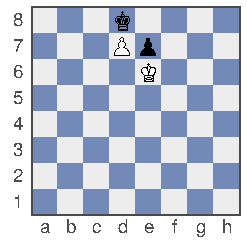
\includegraphics[width=\linewidth]{figures/kinggroup72.pdf}
\caption{Ke6, Pd7 / Kd8, Pe7 (cylinder; the seam plays no part).}
\label{fig:kinggroup72}
\end{subfigure}
\caption{King groups that the convention reads as $0$. (a) and (b) are tr\'ebuchets and real mutual
zugzwangs. (c) is the king group of Puzzle~2: with black to move white wins, but with white to move it is a
draw.}
\label{fig:kings}
\end{figure}

\subsection{When Is the Frozen Tr\'ebuchet Exact?}

A \emph{king group} $Z$ is the two kings and some pawns on a block of files, with no pawns on the neighboring
files (the \emph{buffer}). Pawns change file only by capturing, so the buffer stays empty and no pawn crosses
it. A \emph{decisive event} is a move that creates a passed pawn, or a move inside $Z$.

\begin{theorem}[Validity of the convention; \lab{P}]\label{thm:validity}
Let a king-and-pawn position consist of pawn components and a king group $Z$ with its buffer. Suppose that at
every position before the first decisive event:
\begin{enumerate}
\item[(V1)] the kings never interact with the components: the legal chess moves are exactly the moves of the
  model, en passant included, nobody is in check, and the side to move has a legal move;
\item[(V2)] every decisive event really wins: the side that gets a passed pawn wins the game;
\item[(V3)] every move inside $Z$, by either side, is decisively punished.
\end{enumerate}
Then, with either side to move, the chess result is the normal-play outcome of the pawn components alone, and
there are no draws. If moreover
\begin{enumerate}
\item[(V4)] no two components ever carry passed-pawn threats of opposite sign, and $\BIG$ exceeds every tempo
  count,
\end{enumerate}
then it is also the outcome class of the $\pm\BIG$ value of the components.
\end{theorem}

\begin{proof}[Proof sketch]
By (V3) every move in $Z$ loses, so the model is the normal-play sum of the components, a short game without
draws. Its winner $\sigma$ follows a winning strategy and never moves in $Z$. By (V1) every legal move of the
loser is a move of the model, and the loser always has one, so play ends at a decisive event in $\sigma$'s
favour: a passed pawn for $\sigma$, or a forced move of the loser in $Z$. By (V2) and (V3), $\sigma$ wins the
chess game. Under (V4), the argument of Theorem~\ref{thm:hss} gives the same outcome class for $\pm\BIG$.
\end{proof}

The proof shows what the tr\'ebuchet is really for: it turns stalemate into a loss, by always offering the side
without a pawn move a legal, losing move. Each condition can fail: a king walks over to the pawns (V1), a passed
pawn loses its race (V2), white's king moves in Fig.~\ref{fig:kinggroup72} are not punished (V3), and a $+\BIG$
in one component cancels a $-\BIG$ in another (V4; Section~\ref{sec:sums-hss}).

Condition (V3) depends on the other components, but it has a local certificate with horizon $T$: after the
punishing capture, and with all other pawns removed, the punisher promotes within $T$ moves even if the
defender may pass at any time; the defender cannot promote anywhere within $T$ moves; and the defender is never
stalemated in that window. The certificate implies (V3) for that move \lab{P}.

\begin{proposition}[\lab{P}]\label{prop:horizon1}
A punishment with a local certificate of horizon $T=1$ is decisive in every context without a passed pawn.
\end{proposition}

\begin{proof}
A pawn that could promote in one move stands on its seventh rank with no enemy pawn ahead, so it is already
passed.
\end{proof}

\begin{conjecture}[\lab{Conj}]\label{conj:horizon2}
For every $T\ge2$ there is a context without a passed pawn in which the certificate of horizon $T$ fails.
\end{conjecture}

In a real tr\'ebuchet the punisher, after winning the pawn, still needs $T\approx5$--$7$ moves to promote, so
the certificate does not cover every context: we trust its zero only beside slow or locked components.

\subsection{Spare King Moves Are Loopy}

A king that can step back and forth forever without loss is not $0$. It gives its side an unlimited supply of
waiting moves, a loopy game~\cite{WinningWays,Siegel2013}: $\textsf{on}=\game{\textsf{on}}{}$ if only white can
wait, $\textsf{off}=\game{}{\textsf{off}}$ if only black can, and $\textsf{dud}$ if both can. Since
$\textsf{on}$ exceeds every number, $\BIG$ included, any sum plus $\textsf{on}$ is a white win, even when black
has a forced passed pawn. The right rule ends the game at the first decisive event.

\begin{theorem}[Outcomes with spare moves; \lab{P}]\label{thm:loopy}
Let the pawn components form a short game, and let every decisive event end the game.
\begin{enumerate}
\item[(a)] If only white can wait, black wins if and only if black can force a decisive event in its favour
  against a white who may pass at any time. Otherwise white wins.
\item[(b)] If both sides can wait, a side wins if and only if it can force a decisive event in its favour
  against an opponent who may pass at any time. Otherwise the game is drawn.
\end{enumerate}
\end{theorem}

\begin{proof}[Proof sketch]
A side that may pass never suffers from having the move, so a winning strategy never passes and must beat
every pass of the opponent. Induction over the acyclic pawn game gives both parts; in (a) every play is finite,
since black cannot pass.
\end{proof}

So a white shuttle makes the component values irrelevant except for black's forcing threats, and shuttles on
both sides remove all tempo content: positions without threats are draws.

\subsection{The King Group of Puzzle 2 Is Not a Zugzwang}

Inside the convention the group of Fig.~\ref{fig:kinggroup72} is a tr\'ebuchet: each side's move loses a pawn.
With black to move it behaves that way. The d7 pawn attacks c8 and e8, so Kc7 is black's only move, and white
takes e7 and promotes. With white to move, however, the king may play Kd5, Ke5, Kf5 or Kf7. After any of the
first three black wins the d7 pawn, but the white king blockades the e-pawn and the game is drawn; only Kf7
loses. So the group is frozen for black only \lab{C2} (our solver and the Lichess tablebase on the ordinary
board; our solver gives the same move values on the cylinder). It is a mutual zugzwang only inside the
convention, where dropping a pawn means losing.

\subsection{How Often Does the Convention Fail?}\label{sec:kings-sweep}

We placed every small pawn component beside a tr\'ebuchet, on $6\times6$ and $7\times6$ cylinders and a
$5\times6$ ordinary board, and solved each position with the kings played out. Of the $500$ components we could
test, $159$ get the wrong outcome \lab{C1}. In $107$ the kings alone are the cause: with frozen kings the
solver reproduces the CGT outcome. The other $52$ are failures of the pawn convention itself,
$18$ through en passant and $34$ because a passed pawn does not actually win its race. Small boards are a
stress test, since the kings are never far from the pawns. On the $8\times8$ board they stand farther away, but
they still matter: in $94$ tablebase-checked positions beside a tr\'ebuchet, $41$ of the $449$ king moves draw
and $7$ win \lab{C1}, where the convention says that every king move loses. This is why the headline values of
this paper are later checked against real chess.
